%!TEX root = proj.tex

\subsection{Weather data}\label{ch:desc_weather}
Historical weather data was obtained and prepared as described in \Cref{appx:weather_data_prep}. The preprocessed weather data is a more advanced time series containing several measurements for each time step. \Cref{tab:weather_data_attr} shows the attributes in the weather data set, and \Cref{tab:weather_data_example} shows an example of the data set.

\begin{table}[!ht]
    \center
    \begin{tabular}{p{.7in}p{4.5in}}        
        Attribute & Description \\
        \hline 
        \hline 
        \gls{t_i} & \glsdesc{t_i} \\
        \hline         
        \gls{temp_i} &  \glsdesc{temp_i}  \\
        \hline         
        \gls{pptn_i} & \glsdesc{pptn_i}\\
        \hline         
        \gls{rh_i} & \glsdesc{rh_i} \\
        \hline         
        \gls{ws_i} & \glsdesc{ws_i} \\
        \hline         
        \gls{cond_i} & \glsdesc{cond_i} \\
    \end{tabular}
    \caption{Attributes in the travel demand data set.}
    \label{tab:weather_data_attr}
\end{table}

\begin{table}[!ht]
    \center
    \begin{tabular}{rlrrrrl}
  & $\mathit{t}$ & $\mathit{temp}$ & $\mathit{pptn}$ & $\mathit{rh}$ & $\mathit{ws}$ & $\mathit{cond}$ \\ 
  \hline
\hline
1 & 2016-10-01 00:00 & 12.00 & 0.00 &  78 & 24.10 & Cloudy \\ 
   \hline
2 & 2016-10-01 00:20 & 12.00 & 0.00 &  88 & 18.50 & Cloudy \\ 
   \hline
3 & 2016-10-01 00:50 & 12.00 & 0.00 &  88 & 16.70 & Cloudy \\ 
   \hline
4 & 2016-10-01 01:00 & 12.00 & 0.00 &  81 & 14.80 & Clear \\ 
   \hline
5 & 2016-10-01 01:20 & 12.00 & 0.00 &  88 & 13.00 & Cloudy \\ 
   \hline
6 & 2016-10-01 01:50 & 13.00 & 0.00 &  88 & 16.70 & Cloudy \\ 
   \hline
7 & 2016-10-01 02:00 & 13.00 & 0.00 &  85 & 20.40 & Cloudy \\ 
   \hline
8 & 2016-10-01 02:20 & 13.00 & 0.00 &  88 & 18.50 & Cloudy \\ 
   \hline
9 & 2016-10-01 02:50 & 12.00 & 0.00 &  88 & 14.80 & Cloudy \\ 
   \hline
10 & 2016-10-01 03:00 & 12.00 & 0.00 &  84 & 13.00 & Cloudy \\ 
  \end{tabular}

    \caption{Example of the weather data set.}
    \label{tab:weather_data_example}
\end{table}

Weather conditions seems quite sparse, e.g.\ as shown in \Cref{fig:weather_hist} rain conditions are only observed $\approx12 \%$ of the time, and show $<3 \%$ of the time. And in the vast majority of time it is raining the rain condition is considered \emph{light}.

\begin{figure}[!ht]
    \center
    % !TEX encoding = UTF-8 Unicode
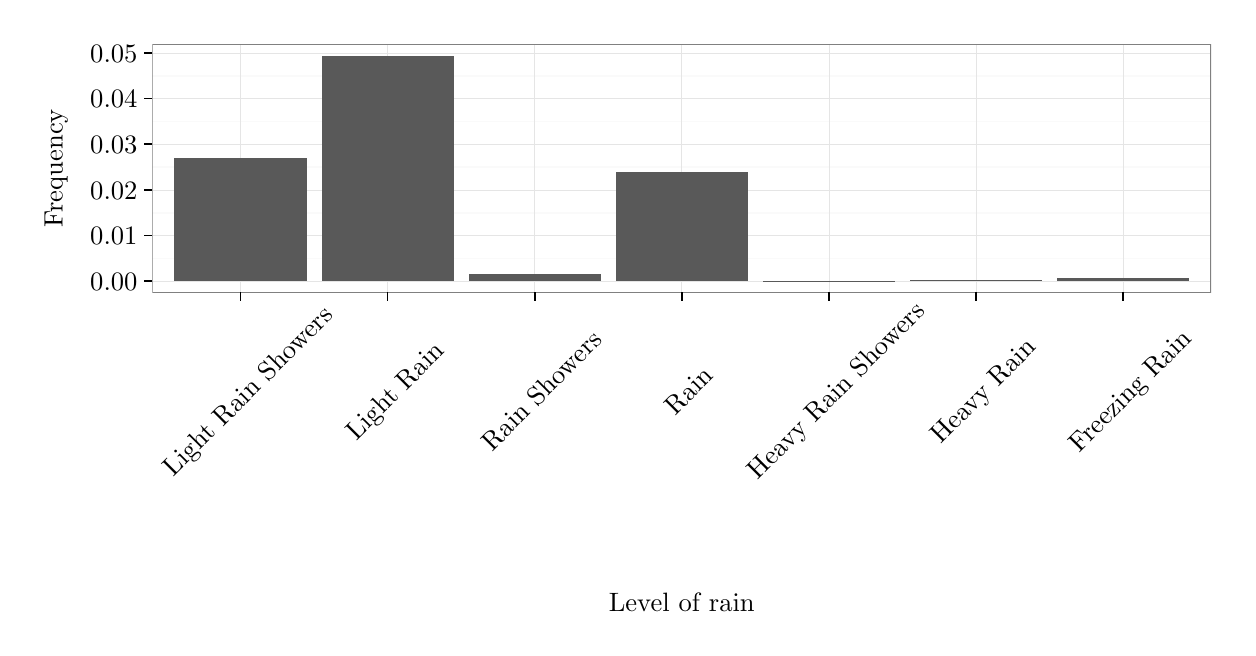
\begin{tikzpicture}[x=1pt,y=1pt]
\definecolor{fillColor}{RGB}{255,255,255}
\path[use as bounding box,fill=fillColor,fill opacity=0.00] (0,0) rectangle (433.62,216.81);
\begin{scope}
\path[clip] (  0.00,  0.00) rectangle (433.62,216.81);
\definecolor{drawColor}{RGB}{255,255,255}
\definecolor{fillColor}{RGB}{255,255,255}

\path[draw=drawColor,line width= 0.6pt,line join=round,line cap=round,fill=fillColor] (  0.00,  0.00) rectangle (433.62,216.81);
\end{scope}
\begin{scope}
\path[clip] ( 45.07,121.14) rectangle (427.62,210.81);
\definecolor{fillColor}{RGB}{255,255,255}

\path[fill=fillColor] ( 45.07,121.14) rectangle (427.62,210.81);
\definecolor{drawColor}{gray}{0.98}

\path[draw=drawColor,line width= 0.6pt,line join=round] ( 45.07,133.46) --
	(427.62,133.46);

\path[draw=drawColor,line width= 0.6pt,line join=round] ( 45.07,149.95) --
	(427.62,149.95);

\path[draw=drawColor,line width= 0.6pt,line join=round] ( 45.07,166.45) --
	(427.62,166.45);

\path[draw=drawColor,line width= 0.6pt,line join=round] ( 45.07,182.94) --
	(427.62,182.94);

\path[draw=drawColor,line width= 0.6pt,line join=round] ( 45.07,199.43) --
	(427.62,199.43);
\definecolor{drawColor}{gray}{0.90}

\path[draw=drawColor,line width= 0.2pt,line join=round] ( 45.07,125.22) --
	(427.62,125.22);

\path[draw=drawColor,line width= 0.2pt,line join=round] ( 45.07,141.71) --
	(427.62,141.71);

\path[draw=drawColor,line width= 0.2pt,line join=round] ( 45.07,158.20) --
	(427.62,158.20);

\path[draw=drawColor,line width= 0.2pt,line join=round] ( 45.07,174.69) --
	(427.62,174.69);

\path[draw=drawColor,line width= 0.2pt,line join=round] ( 45.07,191.18) --
	(427.62,191.18);

\path[draw=drawColor,line width= 0.2pt,line join=round] ( 45.07,207.67) --
	(427.62,207.67);

\path[draw=drawColor,line width= 0.2pt,line join=round] ( 76.95,121.14) --
	( 76.95,210.81);

\path[draw=drawColor,line width= 0.2pt,line join=round] (130.08,121.14) --
	(130.08,210.81);

\path[draw=drawColor,line width= 0.2pt,line join=round] (183.22,121.14) --
	(183.22,210.81);

\path[draw=drawColor,line width= 0.2pt,line join=round] (236.35,121.14) --
	(236.35,210.81);

\path[draw=drawColor,line width= 0.2pt,line join=round] (289.48,121.14) --
	(289.48,210.81);

\path[draw=drawColor,line width= 0.2pt,line join=round] (342.61,121.14) --
	(342.61,210.81);

\path[draw=drawColor,line width= 0.2pt,line join=round] (395.74,121.14) --
	(395.74,210.81);
\definecolor{fillColor}{gray}{0.35}

\path[fill=fillColor] ( 53.04,125.22) rectangle (100.86,169.63);

\path[fill=fillColor] (106.18,125.22) rectangle (153.99,206.73);

\path[fill=fillColor] (159.31,125.22) rectangle (207.12,127.74);

\path[fill=fillColor] (212.44,125.22) rectangle (260.26,164.71);

\path[fill=fillColor] (265.57,125.22) rectangle (313.39,125.34);

\path[fill=fillColor] (318.70,125.22) rectangle (366.52,125.59);

\path[fill=fillColor] (371.83,125.22) rectangle (419.65,126.48);
\definecolor{drawColor}{gray}{0.50}

\path[draw=drawColor,line width= 0.6pt,line join=round,line cap=round] ( 45.07,121.14) rectangle (427.62,210.81);
\end{scope}
\begin{scope}
\path[clip] (  0.00,  0.00) rectangle (433.62,216.81);
\definecolor{drawColor}{RGB}{0,0,0}

\node[text=drawColor,anchor=base east,inner sep=0pt, outer sep=0pt, scale=  0.96] at ( 39.67,121.91) {0.00};

\node[text=drawColor,anchor=base east,inner sep=0pt, outer sep=0pt, scale=  0.96] at ( 39.67,138.40) {0.01};

\node[text=drawColor,anchor=base east,inner sep=0pt, outer sep=0pt, scale=  0.96] at ( 39.67,154.89) {0.02};

\node[text=drawColor,anchor=base east,inner sep=0pt, outer sep=0pt, scale=  0.96] at ( 39.67,171.39) {0.03};

\node[text=drawColor,anchor=base east,inner sep=0pt, outer sep=0pt, scale=  0.96] at ( 39.67,187.88) {0.04};

\node[text=drawColor,anchor=base east,inner sep=0pt, outer sep=0pt, scale=  0.96] at ( 39.67,204.37) {0.05};
\end{scope}
\begin{scope}
\path[clip] (  0.00,  0.00) rectangle (433.62,216.81);
\definecolor{drawColor}{RGB}{0,0,0}

\path[draw=drawColor,line width= 0.6pt,line join=round] ( 42.07,125.22) --
	( 45.07,125.22);

\path[draw=drawColor,line width= 0.6pt,line join=round] ( 42.07,141.71) --
	( 45.07,141.71);

\path[draw=drawColor,line width= 0.6pt,line join=round] ( 42.07,158.20) --
	( 45.07,158.20);

\path[draw=drawColor,line width= 0.6pt,line join=round] ( 42.07,174.69) --
	( 45.07,174.69);

\path[draw=drawColor,line width= 0.6pt,line join=round] ( 42.07,191.18) --
	( 45.07,191.18);

\path[draw=drawColor,line width= 0.6pt,line join=round] ( 42.07,207.67) --
	( 45.07,207.67);
\end{scope}
\begin{scope}
\path[clip] (  0.00,  0.00) rectangle (433.62,216.81);
\definecolor{drawColor}{RGB}{0,0,0}

\path[draw=drawColor,line width= 0.6pt,line join=round] ( 76.95,118.14) --
	( 76.95,121.14);

\path[draw=drawColor,line width= 0.6pt,line join=round] (130.08,118.14) --
	(130.08,121.14);

\path[draw=drawColor,line width= 0.6pt,line join=round] (183.22,118.14) --
	(183.22,121.14);

\path[draw=drawColor,line width= 0.6pt,line join=round] (236.35,118.14) --
	(236.35,121.14);

\path[draw=drawColor,line width= 0.6pt,line join=round] (289.48,118.14) --
	(289.48,121.14);

\path[draw=drawColor,line width= 0.6pt,line join=round] (342.61,118.14) --
	(342.61,121.14);

\path[draw=drawColor,line width= 0.6pt,line join=round] (395.74,118.14) --
	(395.74,121.14);
\end{scope}
\begin{scope}
\path[clip] (  0.00,  0.00) rectangle (433.62,216.81);
\definecolor{drawColor}{RGB}{0,0,0}

\node[text=drawColor,rotate= 45.00,anchor=base,inner sep=0pt, outer sep=0pt, scale=  0.96] at ( 81.63, 83.47) {Light Rain Showers};

\node[text=drawColor,rotate= 45.00,anchor=base,inner sep=0pt, outer sep=0pt, scale=  0.96] at (134.76, 83.47) {Light Rain};

\node[text=drawColor,rotate= 45.00,anchor=base,inner sep=0pt, outer sep=0pt, scale=  0.96] at (187.89, 83.47) {Rain Showers};

\node[text=drawColor,rotate= 45.00,anchor=base,inner sep=0pt, outer sep=0pt, scale=  0.96] at (241.02, 83.47) {Rain};

\node[text=drawColor,rotate= 45.00,anchor=base,inner sep=0pt, outer sep=0pt, scale=  0.96] at (294.15, 83.47) {Heavy Rain Showers};

\node[text=drawColor,rotate= 45.00,anchor=base,inner sep=0pt, outer sep=0pt, scale=  0.96] at (347.29, 83.47) {Heavy Rain};

\node[text=drawColor,rotate= 45.00,anchor=base,inner sep=0pt, outer sep=0pt, scale=  0.96] at (400.42, 83.47) {Freezing Rain};
\end{scope}
\begin{scope}
\path[clip] (  0.00,  0.00) rectangle (433.62,216.81);
\definecolor{drawColor}{RGB}{0,0,0}

\node[text=drawColor,anchor=base,inner sep=0pt, outer sep=0pt, scale=  0.96] at (236.35,  6.00) {Level of rain};
\end{scope}
\begin{scope}
\path[clip] (  0.00,  0.00) rectangle (433.62,216.81);
\definecolor{drawColor}{RGB}{0,0,0}

\node[text=drawColor,rotate= 90.00,anchor=base,inner sep=0pt, outer sep=0pt, scale=  0.96] at ( 12.61,165.98) {Frequency};
\end{scope}
\end{tikzpicture}

    \caption{Frequency of different levels of rain.}
    \label{fig:weather_hist}
\end{figure}